\section{Communication technologies in Automotive Domain}
It is important to note that the incorporation of Ethernet as an in-vehicle networking system does not imply that traditional communication networks such as CAN, LIN, and MOST are rendered obsolete. Because these networks are robust, inexpensive, time-tested, and provide necessary performance for many applications, Automotive Ethernet will not completely replace them, but will supplement them to provide even more cost, performance, and feature benefits. Table \ref{tab:Comparison_Automotive_Networks} shows the important characteristics of automotive networks in comparison with the Ethernet.
\begin{center}
\begin{tabular}{|c|c|c|c|c|c|c}
\hline
\textbf{Property} & \textbf{Ethernet} & \textbf{CAN} & \textbf{FlexRay} & \textbf{MOST} & \textbf{LIN}\\
\hline
Bandwidth(Mb/s) & \textgreater 100 & 1 & 20 & 150 & 0.02\\
\hline
Nodes & Scalable & 30 & 22 & 64 & 16\\
\hline
Network Length & 15m per link & 40m & 24m & 1280m & 40m\\
\hline
%Media Access Control & Full-duplex contention less & Non-destructive arbitration & Time-triggered & Time-triggered & Time-triggered\\
Topologies & Star, Tree & Bus& Bus,start & Ring,Star & Bus\\
\hline
Cost & High& Low& Low& High& Very low\\
\hline
Cabling & UTP & UTP & UTP & Optical,UTP & 1-wire\\

\hline
\end{tabular}
\captionof{table}{Comparison of important characteristics of automotive networks \cite[p.202]{b1}}
\label{tab:Comparison_Automotive_Networks}
\end{center}

\section{Role of Ethernet in the Automotive Domain}
Insert text here.

\section{Ethernet as backbone in vehicles}
Insert text here.
\begin{figure}[!htb]
	\centering
		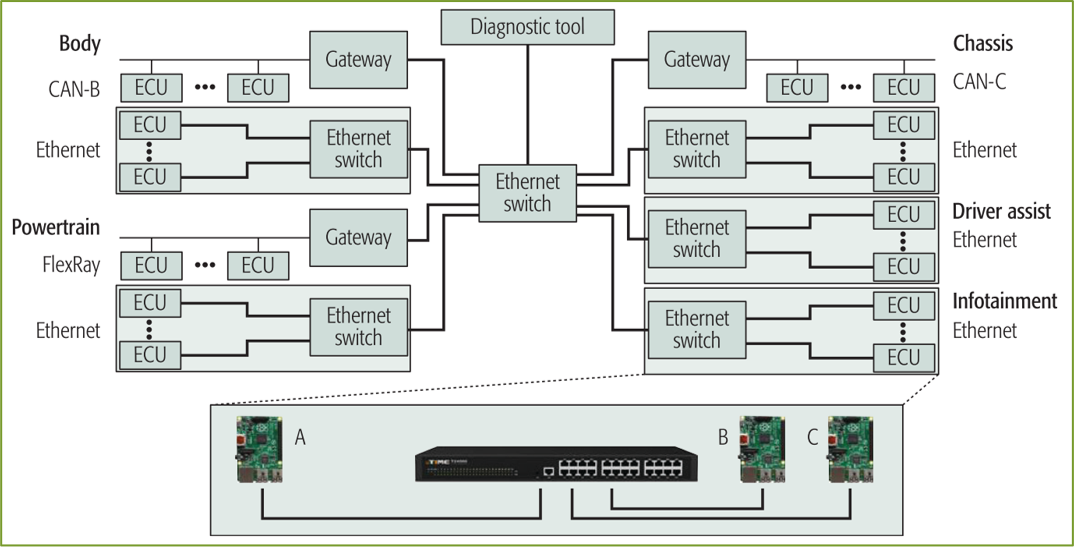
\includegraphics[width=1\textwidth]{images/Switched_Ethernet_backbone.png}
	\caption{Ethernet as a backbone \cite{b5.0}}
	\label{fig:Switched_Ethernet_backbone}
\end{figure}


\section{Service Oriented Architecture}
Insert text here.	

\section{Middleware technologies in automotive domain}
Briefly describe about the need and existing technologies. (SOME/IP, DDS)

\subsection{SOME/IP}
"`Scalable service Oriented MiddlewarE over IP"' abbreviated SOME/IP represents a middleware that was created for automotive use cases \cite{b1.1}. The compatibility with AUTOSAR was a necessity regarding SOME/IP at least on wire-format level \cite{b1.1}. SOME/IP communication is an exchange of messages between different devices like ECUs over IP \cite{b1.1}. There are more patterns available for basic SOME/IP communication \cite{b1.1}.

\begin{figure}[!htb]
	\centering
		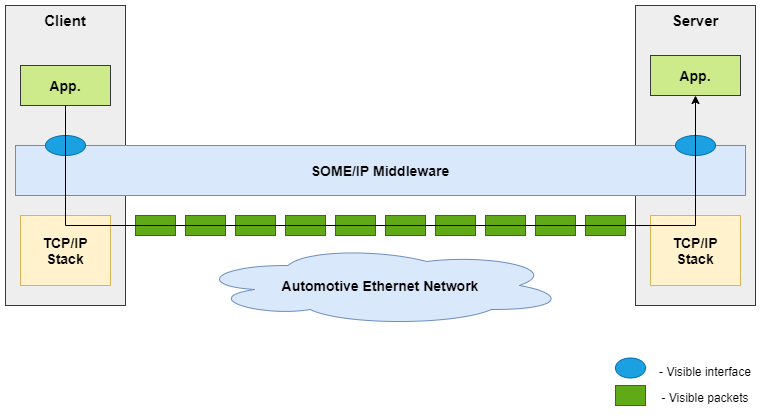
\includegraphics[width=1\textwidth]{images/SOMEIP_Middleware.png}
	\caption{SOA representation with SOME/IP middleware}
	\label{fig:SOMEIP_Middleware}
\end{figure}


\subsubsection{Communication methods}
Brief description of the communication methods. Explain in brief about each of the types.

\begin{itemize}
	\item Request-Response
	\begin{figure}[!htb]
	\centering
		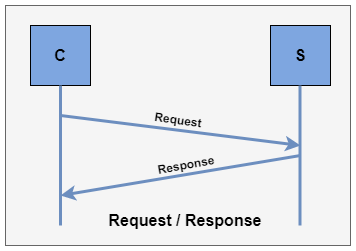
\includegraphics{images/Request-response.png}
	\caption{Request-Response communication type}
	\label{fig:Request-response}
\end{figure}
\end{itemize}


\begin{figure}[!htb]
	\centering
		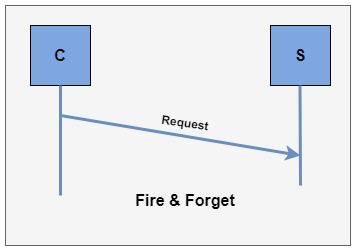
\includegraphics{images/fire-forget.png}
	\caption{Fire \& Forget communication type}
	\label{fig:fire-forget}
\end{figure}

\begin{figure}[!htb]
	\centering
		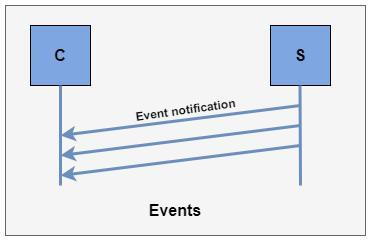
\includegraphics{images/Events.png}
	\caption{Events communication type}
	\label{fig:Events}
\end{figure}

\begin{figure}[!htb]
	\centering
		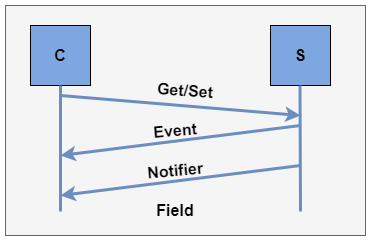
\includegraphics{images/Field.png}
	\caption{Fields communication type}
	\label{fig:Field}
\end{figure}








